
We evaluate \DyNACS{} as a zero-shot learning-guided optimizer within each problem type. Unless otherwise specified, a single model trained on uniformly distributed 1K-node synthetic instances is directly tested on benchmark \TSP{} and \CVRP{} instances with different scales, structures, and distributions. Conventional neural combinatorial optimization often trains and tests on matched synthetic distributions, or trains different models for different scales. Our evaluation instead asks whether state-aware guidance transfers beyond the training distribution while preserving the efficiency and reliability of the underlying ACO search.

The evaluation follows the method's dependency chain. The main benchmark comparison tests whether the full model improves zero-shot performance against classical solvers, neural routing solvers, and neural-guided ACO baselines. The trajectory-diversity study asks whether population-aware guidance improves the state-aware \DyNACO{} base model inside the same ACO environment. The ablations test dynamic guidance, SRR credit assignment, pheromone stabilization, and inference controls. The final analyses report runtime, neural overhead, training efficiency, and learned guidance behavior to clarify how the method scales in practice.

\subsection{Experimental Setup}
\label{sec:setup}

\smallskip\noindent\textbf{Training setup.}
All experiments use a fixed random seed and one deterministic run per instance. Training instances are generated online, with coordinates sampled uniformly from $[0,1]^2$, yielding 320 training instances in total (32 per epoch $\times$ 10 epochs). We train with PPO on a single RTX 5090 GPU and Ryzen 9 7950X CPU with 16 cores. Default \DyNACS{} hyperparameters are summarized in Table~\ref{tab:hyperparams}, and baseline configurations are detailed in Appendix~\ref{app:setup}.

\smallskip\noindent\textbf{Benchmark datasets.}
For the main zero-shot evaluation, we follow a benchmark protocol designed to test generalization. The \TSP{} test suite includes instances from TSPLIB~\cite{tsplib}, National TSP~\cite{nationaltsp}, VLSI TSP~\cite{vlsitsp}, and the 8th DIMACS Implementation Challenge for TSP~\cite{dimacs8tsp}. These datasets cover geographic, industrial, clustered, and benchmark-generated structures. The \CVRP{} test suite includes instances from CVRPLIB~\cite{cvrplib}, including Set X and large-scale AGS instances~\cite{ags}. We include only standard Euclidean instances with available best-known solutions and without additional side constraints such as fixed edges, fixed route numbers, or duration limits.

The benchmark suite is substantially more challenging than synthetic testing on the training distribution. The training distribution contains only uniform 1K-node instances, whereas the test suite contains benchmark instances with diverse structures and scales. Strong performance on this suite indicates zero-shot transfer across both scale and distribution.

\smallskip\noindent\textbf{Candidate graph and backend.}
The candidate graph is a symmetric $K$-nearest-neighbor graph with $K{=}32$, with ties broken by node index. A backup list of 64 additional neighbors is maintained for fallback~\cite{ACOTSP-MF}. For \TSP{}, the backend follows the ACO design based on perturbations from~\cite{faco}. For \CVRP{}, we use a capacity-aware version of the same backend with scope-restricted refinement, described in Appendix~\ref{app:cvrp}.

\smallskip\noindent\textbf{Baselines.}
We compare with four groups of methods. First, we include simple construction heuristics, including Nearest Neighbor and Random Insertion. These baselines are important because recent evaluations of generalization show that many neural solvers can degrade below simple heuristics under benchmark distribution shift. Second, we include strong classical solvers, including LKH-3~\cite{lkhtsp,lkhcvrp} for \TSP{} and HGS~\cite{hgs} and AILS-II~\cite{ails2} for \CVRP{}. Third, we compare with representative neural routing solvers, including BQ~\cite{bq}, LEHD~\cite{lehd}, SIL~\cite{sil}, ICAM~\cite{icam}, ELG~\cite{elg}, INViT~\cite{invit}, L2R~\cite{l2r}, DGL~\cite{dgl}, ReLD~\cite{reld}, L2C-Insert~\cite{l2c}, H-TSP~\cite{htsp}, DACT~\cite{dact}, NeuOpt~\cite{neuopt}, DRHG~\cite{drhg}, and Fast T2T~\cite{fastt2t}. Finally, we compare with neural-guided ACO methods, including DeepACO~\cite{deepaco}, GFACS~\cite{gfacs}, GTG-ACO~\cite{gtgaco}, and HeatACO~\cite{heataco}.

We also include the unguided ACO backend as a direct ablation baseline. Because \DyNACO{}, \DyNACS{}, and the unguided backend share the same candidate graph, perturbation mechanism, refinement procedure, and search budget, this comparison isolates the contribution of neural guidance.

\smallskip\noindent\textbf{Metrics.}
We report three complementary metrics. \emph{Effectiveness} is measured by the average optimality gap to the best-known solution (BKS):
\begin{equation}
\mathrm{Gap} =
\frac{\mathrm{Obj.}-\mathrm{BKS}}{\mathrm{BKS}}
\times 100%.
\end{equation}
\emph{Efficiency} is measured by wall-clock inference time. \emph{Reliability} is measured by the number of successfully solved instances. A method is considered unsuccessful if it runs out of memory, times out, fails to produce a feasible solution, or suffers severe performance breakdown. Results are grouped into three scale ranges: $(0,1\mathrm{K})$, $[1\mathrm{K},10\mathrm{K})$, and $[10\mathrm{K},100\mathrm{K}]$, with aggregate results also reported.

\subsection{Zero-Shot Generalization on Benchmarks}
\label{sec:main-results}

Table~\ref{tab:exp_proposed} presents the main zero-shot results on \TSP{} and \CVRP{} benchmarks. Unlike the conventional setting where training and testing distributions are matched, all neural methods are evaluated without retraining or fine-tuning on benchmark instances. \DyNACS{} achieves the strongest overall performance among neural methods while solving all instances.

\begin{table}[h]
\centering
\caption{Headline zero-shot results from Table~\ref{tab:exp_proposed}.}
\label{tab:headline-results}
\small
\renewcommand{\arraystretch}{0.85}
\begin{tabular*}{\columnwidth}{@{\extracolsep{\fill}}lcc@{}}
\toprule
Method & \TSP{} Total & \CVRP{} Total \\
\midrule
Best prior neural baseline & 1.71\% / 228 & 4.58\% / 107 \\
ACO backend & 1.82\% / 228 & 3.18\% / 110 \\
\DyNACO{} (single behavior) & 1.48\% / 228 & 3.10\% / 110 \\
\DyNACS{} & \textbf{1.22\% / 228} & \textbf{2.80\% / 110} \\
\bottomrule
\end{tabular*}
\end{table}


\begin{table*}[htbp]
  \centering
  \caption{Experimental Results of the Proposed Evaluation Pipeline}
  \vspace{-0.2cm}
  \tabcolsep=0.185cm
  \begin{threeparttable}
    \begin{tabular}{c|l|ccc|ccc|ccc|cc}
    \toprule[0.5mm]
          & \multicolumn{1}{c|}{\multirow{2}[2]{*}{Method}} & \multicolumn{3}{c|}{(0,1K)} & \multicolumn{3}{c|}{[1K, 10K)} & \multicolumn{3}{c|}{[10K, 100K]} & \multicolumn{2}{c}{Total} \\
\cmidrule{3-13}          &       & Gap   & Time  & \multicolumn{1}{l|}{Solved} & Gap   & Time  & \multicolumn{1}{l|}{Solved} & Gap   & Time  & \multicolumn{1}{l|}{Solved} & Gap   & Solved \\
\cmidrule{1-13}    \multirow{26}[13]{*}{\rotatebox[origin=c]{90}{TSP}} & Nearest Neighbor & 25.29\% & 0.01s & 69/69 & 26.66\% & 0.29s & 109/109 & 25.01\% & 22.60s & 50/50 & 25.88\% &  {{228}/228} \\
          & Random Insertion & 10.60\% &  {{0.00s}} & 69/69 & 15.32\% &  {{0.05s}} & 109/109 & 16.37\% &  {{8.93s}} & 50/50 & 14.12\% &  {{228}/228} \\
          & LKH-3\phantom{$^{\downarrow}$} t=n/3, runs=1 & 0.00\% & 7.88s & 69/69 & 0.01\% & 631.34s & 109/109 & 0.08\% & 14600.50s & 50/50 & 0.03\% &  {{228}/228} \\
          & LKH-3$^{\downarrow}$ t=n/3, runs=1 & 0.00\% & 9.25s & 69/69 & 0.01\% & 600.36s & 109/109 & 0.05\% & 10800.24s & 50/50 &  {{0.02\%}} &  {{228}/228} \\
\cmidrule{2-13}          & BQ    & 5.00\% & 2.51s & 68/69 & 19.03\% & 22.74s & 92/109 & 52.00\% & 187.81s & 4/50  & 14.02\% & 164/228 \\
          & LEHD$^*$ greedy & 4.85\% & 1.01s & 69/69 & 20.13\% & 68.27s & 106/109 & 49.35\% & 1386.01s & 11/50 & 16.19\% & 186/228 \\
          & SIL$^*$ greedy & 8.64\% & 1.69s & 69/69 & 9.83\% & 17.69s & 109/109 & 11.11\% & 430.73s & 50/50 & 9.75\% &  {{228}/228} \\
          & ICAM  & 6.53\% & 0.25s & 69/69 & 16.62\% & 21.57s & 109/109 & 21.34\% & 1050.33s & 19/50 & 13.54\% & 197/228 \\
          & ELG   & 6.05\% & 0.63s & 69/69 & 18.14\% & 88.12s & 108/109 & 21.65\% & 940.35s & 6/50  & 13.70\% & 183/228 \\
          & INViT-3V   & 7.93\% & 2.77s & 69/69 & 12.08\% & 49.03s & 109/109 & 11.52\% & 1079.50s & 42/50 & 10.67\% & 220/228 \\
          & L2R   & 5.89\% & 1.60s & 69/69 & 9.22\% & 15.55s & 109/109 & 8.52\% & 153.11s & 50/50 &  {{8.06\%}} &  {{228}/228}   \\
          & DGL   & 6.53\% & 1.17s & 69/69 & 11.32\% & 11.67s & 109/109 & 11.14\% & 58.62s & 25/50 & 9.67\% & 203/228 \\
          & L2C-Insert$^*$ greedy & 4.39\% & 1.51s & 69/69 & 18.12\% & 15.34s & 109/109 & 30.94\% & 145.17s & 50/50 & 16.77\% &  {{228}/228}   \\
\cmidrule{2-13}          & H-TSP & 6.16\% &  {{0.61s}} & 36/69 & 11.62\% &  {{3.15s}} & 100/109 & 12.29\% &  {{21.44s}} & 40/50 & 10.65\% & 176/228 \\
\cmidrule{2-13}          & DACT T=1K & 16.37\% & 39.84s & 69/69 & 26.58\% & 261.73s & 83/109 & /     & /     & 0/50  & 21.94\% & 152/228 \\
          & NeuOpt T=1K & 19.90\% & 81.22s & 46/69 & /     & /     & 0/109 & /     & /     & 0/50  & 19.90\% & 46/228 \\
\cmidrule{2-13}          & L2C-Insert$^*$ T=1K & 1.08\% & 381.55s & 69/69 & 9.80\% & 479.98s & 109/109 & 29.15\% & 615.19s & 50/50 & 11.41\% &  {{228}/228}   \\
          & LEHD$^*$ RRC1K & 1.73\% & 498.40s & 69/69 & 10.87\% & 1634.51s & 109/109 & 24.02\% & 2769.86s & 9/50  & 8.13\% & 187/228 \\
          & SIL$^*$ PRC1K & 0.80\% & 883.87s & 69/69 & 2.58\% & 2880.46s & 109/109 & 4.55\% & 4933.45s & 50/50 & 2.47\% &  {{228}/228} \\
          & DRHG T=1K & 0.10\% & 769.53s & 69/69 & 1.46\% & 2857.55s & 109/109 & 4.46\% & 3004.28s & 50/50 &  {{1.71\%}} &  {{228}/228}   \\
          & Fast T2T T\textsubscript{s}=10, T\textsubscript{g}=10 & 10.46\% & 1.41s & 45/69 & /     & /     & 0/109 & /     & /     & 0/50  & 10.46\% & 45/228 \\
\cmidrule{2-13}          & GFACS$^{\dagger}$ T=100, K=100 & 31.64\% & 166.94s & 66/69 & 86.77\% & 2601.13s & 22/109 & /     & /     & 0/50  & 45.42\% & 88/228 \\
          & GFACS$^{\ddagger}$ T=100, K=100 & 0.72\% & 174.21s & 69/69 & 3.76\% & 9142.93s & 83/109 & /     & /     & 0/50  & 2.38\% & 152/228 \\
    \midrule

\cmidrule{2-13}
          & ACO
          & 0.28\% & -- & 69/69
          & 1.59\% & -- & 109/109
          & 4.44\% & -- & 50/50
          & 1.82\% & 228/228 \\

          & \DyNACO{}
          & 0.23\% & 0.59s & 69/69
          & 1.22\% & 1.58s & 109/109
          & 3.99\% & 12.14s & 50/50
          & 1.48\% & 228/228 \\

          & \DyNACS{}
          & \textbf{0.14\%} & 0.86s & \textbf{69/69}
          & \textbf{0.95\%} & 3.39s & \textbf{109/109}
          & \textbf{3.33\%} & 34.45s & \textbf{50/50}
          & \textbf{1.22\%} & \textbf{228/228} \\


\midrule
    \midrule
    \multirow{25}[13]{*}{\rotatebox[origin=c]{90}{CVRP}} & Nearest Neighbor & 21.17\% & 0.03s & 99/99 & 15.18\% & 1.08s & 5/5   & 11.80\% & 14.63s & 6/6   & 20.39\% &  {{110}/110} \\
          & Random Insertion & 75.00\% & 0.00s & 36/99 & /     & /     & 0/5   & /     & /     & 0/6   & 75.00\% & 36/110 \\
          & HGS t=n/3 & 0.29\% & 111.24s & 99/99 & 3.59\% & 1428.41s & 5/5   & 7.86\% & 6926.41s & 6/6   & 0.85\% &  {{110}/110} \\
          & AILS-II t=n/3 & 0.57\% & 133.95s & 99/99 & 1.58\% & 1388.42s & 5/5   & 1.58\% & 5646.48s & 6/6   &  {{0.68\%}} &  {{110}/110} \\
\cmidrule{2-13}          & BQ   & 8.87\% & 3.63s & 99/99 & 20.28\% & 39.97s & 5/5   & 41.52\% & 202.69s & 5/6   & 10.89\% & 109/110 \\
          & LEHD$^*$ greedy & 11.25\% & 1.53s & 98/99 & 19.22\% & 99.43s & 5/5   & 32.80\% & 852.02s & 2/6   & 12.04\% & 105/110 \\
          & SIL$^*$ greedy & 40.04\% & 2.48s & 65/99 & 16.09\% & 26.86s & 5/5   & 10.81\% & 146.83s & 6/6   & 36.16\% & 76/110 \\
          & ICAM  & 5.00\% & 0.42s & 99/99 & 11.69\% & 32.32s & 5/5   & /     & /     & 0/6   & 5.32\% & 104/110 \\
          & ELG   & 8.03\% & 1.29s & 99/99 & 18.51\% & 30.21s & 5/5   & 29.38\% & 133.08s & 2/6   & 8.93\% & 106/110 \\
          & INViT-3V   & 13.15\% & 4.72s & 99/99 & 19.03\% & 77.33s & 5/5   & 23.91\% & 496.25s & 5/6   & 13.91\% & 109/110 \\
          & L2R   & 8.16\% & 2.49s & 99/99 & 11.62\% & 23.99s & 5/5   & 11.08\% & 97.12s & 6/6   & 8.48\% &  {{110}/110}   \\
          & DGL   & 15.27\% & 2.22s & 99/99 & 17.96\% & 22.60s & 5/5   & 18.69\% & 78.64s & 5/6   & 15.55\% & 109/110 \\
          & ReLD  & 4.10\% & 0.41s & 99/99 & 10.22\% & 5.29s & 5/5   & 11.27\% & 28.87s & 3/6   &  {{4.58\%}} & 107/110 \\
          & L2C-Insert$^*$ greedy & 6.87\% & 2.73s & 99/99 & 22.37\% & 616.75s & 5/5   & 49.41\% & 5525.71s & 2/6   & 8.40\% & 106/110 \\
\cmidrule{2-13}          & DACT T=1K & 16.42\% & 246.51s & 74/99 & 17.70\% & 479.82s & 1/5   & /     & /     & 0/6   & 16.44\% & 75/110 \\
          & NeuOpt T=1K & 26.93\% & 571.14s & 36/99 & /     & /     & 0/5   & /     & /     & 0/6   & 26.93\% & 36/110 \\
\cmidrule{2-13}          & L2C-Insert$^*$ T=1K & 3.21\% & 344.05s & 99/99 & 18.87\% & 6166.21s & 5/5   & 44.29\% & 32754.86s & 2/6   & 4.72\% & 106/110 \\
          & LEHD$^*$ RRC1K & 3.58\% & 796.15s & 99/99 & 11.73\% & 2043.74s & 5/5   & 21.98\% & 2820.28s & 2/6   & 4.32\% & 106/110 \\
          & SIL$^*$ PRC1K  & 21.38\% & 1307.97s & 99/99 & 8.28\% & 3471.69s & 5/5   & 7.40\% & 4251.88s & 6/6   & 20.02\% &  {{110}/110}   \\
          & DRHG T=1K & 11.11\% & 1114.60s & 99/99 & 17.95\% & 2529.12s & 5/5   & 16.95\% & 5376.37s & 6/6   & 11.74\% &  {{110}/110}   \\
\cmidrule{2-13}          & GFACS$^{\dagger}$ T=100, K=100 & 36.83\% & 437.38s & 99/99 & 34.09\% & 9654.33s & 3/5   & /     & /     & 0/6   & 36.75\% & 102/110 \\
          & GFACS$^{\ddagger}$ T=100, K=100 & 2.60\% & 405.81s & 99/99 & 7.65\% & 14884.94s & 4/5   & /     & /     & 0/6   & 2.80\% & 103/110 \\
    \midrule

\cmidrule{2-13}
          & ACO
          & 2.83\% & -- & 99/99
          & 5.33\% & -- & 5/5
          & 7.16\% & -- & 6/6
          & 3.18\% & 110/110 \\

          & \DyNACO{}
          & 2.77\% & 1.64s & 99/99
          & 5.01\% & 7.50s & 5/5
          & 6.98\% & 27.64s & 6/6
          & 3.10\% & 110/110 \\

          & \DyNACS{} (ours)
          & \textbf{2.42\%} & -- & \textbf{99/99}
          & \textbf{4.82\%} & -- & \textbf{5/5}
          & \textbf{6.98\%} & -- & \textbf{6/6}
          & \textbf{2.80\%} & \textbf{110/110} \\



    \bottomrule[0.5mm]
    \end{tabular}%
    \begin{tablenotes}
      \footnotesize
      \item[$\downarrow$] $Initial\_Period$ is set as 1K, rather than the original value DIMENSION/2.
      \item[$*$]  The NRS supports more than one inference strategy.
      \item[$\dagger$] GFACS without local search at the last generation. The output solution is the best of the population at the last generation.
      \item[$\ddagger$] The original version of GFACS\@. The output solution is the best in history (all after local search). 
      
    \end{tablenotes}
    \end{threeparttable}
    \vspace{-0.6cm}
  \label{tab:exp_proposed}%
\end{table*}%

\smallskip\noindent\textbf{TSP.}
On \TSP{}, \DyNACS{} achieves the best aggregate gap among neural methods while solving all 228 instances. The advantage is most visible in the medium and large groups, where several end-to-end neural solvers lose instances or degrade sharply. Against the shared ACO backend, the gain is smaller but consistent, showing that learned guidance improves the same search environment under the matched evaluation budget.

\smallskip\noindent\textbf{CVRP.}
On \CVRP{}, \DyNACS{} also gives the best aggregate neural result and solves all 110 instances. The gain over the ACO backend is larger than on \TSP{} in the total column, consistent with the role of multiple learned behaviors in capacity-constrained search, where local decisions are more heterogeneous. \DyNACS{} improves quality while preserving full reliability.

\smallskip\noindent\textbf{Comparison with simple heuristics.}
Nearest Neighbor and Random Insertion test whether neural methods provide value beyond simple handcrafted rules. \DyNACS{} substantially outperforms these heuristics on both problems while preserving full reliability. Several neural baselines degrade below simple heuristics under benchmark distribution shift, highlighting the gap between synthetic-distribution performance and zero-shot benchmark deployment.

\smallskip\noindent\textbf{Scalability of neural baselines.}
The failures and high runtimes of several neural baselines are largely explained by their inference structure. End-to-end constructive policies~\cite{attentionmodel,pomo,bq,lehd,invit,sigd} are usually trained on small instances and often rely on quadratic attention in the number of nodes. When applied directly to larger benchmarks, they face both scale shift and memory pressure. Neural ACO baselines encounter a related dense bottleneck because they materialize heatmap or pheromone-prior matrices in $\mathbb{R}^{N\times N}$ and then use them inside an ACO loop. Decomposition and hierarchical methods such as GLOP~\cite{glop}, H-TSP~\cite{htsp}, SIL~\cite{sil}, and LEHD~\cite{lehd} mitigate this issue, but their global context modules or repeated subproblem calls can still become expensive at extreme scales. In contrast, \DyNACS{} keeps both neural inference and search state on a sparse $K$-NN graph, so the learned component scales with $nK$ rather than a dense edge matrix.

\smallskip\noindent\textbf{Comparison with classical solvers.}
Classical solvers such as LKH-3, HGS, and AILS-II remain stronger in absolute solution quality, reflecting decades of specialized engineering. The learning question in this paper is whether a neural policy can improve a scalable ACO backend under zero-shot evaluation. Table~\ref{tab:exp_proposed} shows consistent gains while keeping reliability at 100\% on both problem families.

\subsection{Effect of Trajectory-Diverse Guidance}
\label{sec:trajectory-diverse-effect}

Table~\ref{tab:trajectory-diverse-effect} compares the three stages of the search system under the same backend and budget. The unguided backend gives the shared ACO environment. \DyNACO{} adds state-aware guidance, reducing the static-heatmap mismatch by updating the transition prior from the current pheromone and incumbent state. \DyNACS{} keeps the same dynamic state representation and lets different ant groups follow behavior-conditioned trajectory distributions in the same colony. The additional reduction from \DyNACO{} to \DyNACS{} connects the improvement to population-level diversity within the observed search state.

\begin{table}[h]
\centering
\caption{Aggregate zero-shot effect of trajectory-diverse guidance from Table~\ref{tab:exp_proposed}.}
\label{tab:trajectory-diverse-effect}
\small
\renewcommand{\arraystretch}{0.85}
\begin{tabular*}{\columnwidth}{@{\extracolsep{\fill}}lcc@{}}
\toprule
Method & \TSP{} Gap & \CVRP{} Gap \\
\midrule
ACO backend & 1.82\%  & 3.18\%  \\
\DyNACO{} (single behavior) & 1.48\% & 3.10\%  \\
\DyNACS{} & \textbf{1.22\%}  & \textbf{2.80\%} \\
\bottomrule
\end{tabular*}
\end{table}

\subsection{Zero-Shot Comparison with Neural-Guided ACO}
\label{sec:neural-aco-comparison}

Table~\ref{tab:neural-aco} compares \DyNACS{} with prior neural-guided ACO methods at their maximum reported scales. Existing neural ACO methods mainly use static heatmaps or static heuristic priors. \DyNACS{} updates guidance throughout the search trajectory and keeps several learned transition priors active inside one shared colony. The comparison supports the central claim that neural guidance should interact with the ACO trajectory as it unfolds, both through state adaptation and through population-level search diversity.


\begin{table}[h]
\centering
\small
\renewcommand{\arraystretch}{0.85}
\caption{Comparison with neural-guided ACO methods at their maximum reported scale. HeatACO~\cite{heataco} combines ACO with other pretrained heatmap models~\cite{attgcn, dimes, utsp, difusco}.}
\label{tab:neural-aco}
\resizebox{\columnwidth}{!}{%
\begin{tabular}{lcccccc}
\toprule
& \multicolumn{2}{c}{\TSP{}1K} & \multicolumn{2}{c}{\TSP{}10K} & \multicolumn{2}{c}{\CVRP{}1K} \\
\cmidrule(lr){2-3} \cmidrule(lr){4-5} \cmidrule(lr){6-7}
Method & Gap & Time & Gap & Time & Gap & Time \\
\midrule
DeepACO~\cite{deepaco}       & 2.87\% & 66s & -- & -- & 2.40\% & 1.3m \\
GFACS~\cite{gfacs}           & 2.63\% & 66s & -- & -- & 2.11\% & 1.3m \\
GTG-ACO~\cite{gtgaco}        & 2.42\% & -- & -- & -- & -- & -- \\
\midrule
ACO+AttGCN~\cite{attgcn}    & 0.44\% & 5s & 1.27\% & 1.47m & -- & -- \\
ACO+DIMES~\cite{dimes}     & 0.39\% & 6s & 1.15\% & 1.4m & -- & -- \\
ACO+UTSP~\cite{utsp}      & 0.42\% & 6s & -- & -- & -- & -- \\
ACO+DIFUSCO~\cite{difusco}   & 0.23\% & 10s & 1.19\% & 2.89m & -- & -- \\
\midrule
\textbf{\DyNACS{} (ours)}                & \textbf{0.20\%} & 4s & \textbf{0.82\%} & 18s & \textbf{1.04\%} & 19s \\
\bottomrule
\end{tabular}}
\end{table}

\subsection{Credit Assignment and Component Ablations}
\label{sec:ablations}

\smallskip\noindent\textbf{Both dynamic guidance mechanisms are essential.}
Table~\ref{tab:ablation-decoupling} separates the two core parts of dynamic neural guidance. Removing training over full trajectories causes the largest degradation, especially on \TSP{}1K and \TSP{}5K. Removing the representation of the search state also hurts performance across all four columns. The ordering of the rows suggests that trajectory-aware training supplies the larger gain, while state features provide an additional improvement once the policy is trained on full search trajectories.

\begin{table}[h]
\centering
\caption{Decoupling the two mechanisms of dynamic neural guidance. Values are gap (\%) to BKS on 16 instances at I$_{1000}$.}
\label{tab:ablation-decoupling}
\small
\resizebox{\columnwidth}{!}{%
\begin{tabular}{lcccc}
\toprule

Method & TSP1K $\downarrow$ & TSP5K $\downarrow$ & TSP10K $\downarrow$ & CVRP1K $\downarrow$ \\
\midrule
Static only       & 3.65 & 4.87 & 3.56 & 3.00 \\
+ Trajectory-aware Training   & 0.75 & 2.11 & 2.28 & 2.79 \\
+ State-aware Representation  (Full)     & \textbf{0.37} & \textbf{1.24} & \textbf{1.62} & \textbf{2.58} \\
\bottomrule
\end{tabular}
}
\end{table}

\smallskip\noindent\textbf{SRR preserves both training signal and search quality.}
Tables~\ref{tab:srr-training} and~\ref{tab:srr-inference} compare SRR with full local search (FLS) and truncated local search (TLS). FLS can produce strong individual solutions, but it may rewrite the sampled perturbation enough to wash out the model's contribution. TLS preserves more of the policy signal, but leaves solutions under-refined. SRR provides the best trade-off: it runs local search to convergence within the perturbation scope, preserving the causal link between the policy action and the post-refinement reward while maintaining low refinement cost.

\begin{table}[h]
\centering
\caption{Training progress under different refinement strategies. Values are improvement over the untrained model.}
\label{tab:srr-training}
\small
\setlength{\tabcolsep}{0pt}
\renewcommand{\arraystretch}{0.80}
\begin{tabular*}{\columnwidth}{@{\extracolsep{\fill}}lccc@{}}
\toprule
Epoch & SRR $\uparrow$ & TLS $\uparrow$ & FLS $\uparrow$ \\
\midrule
0 (untrained) & 0.000\% & 0.000\% & 0.000\% \\
1 & \textbf{+0.224\%} & +0.099\% & -0.003\% \\
5 & \textbf{+0.432\%} & +0.146\% & -0.016\% \\
9 & \textbf{+0.438\%} & +0.127\% & -0.023\% \\
\midrule
Avg. ACO time & \textbf{2.35s} & 4.33s & 8.03s \\
\bottomrule
\end{tabular*}
\end{table}

\begin{table}[h]
\centering
\caption{Inference quality and runtime under different refinement strategies (TSP-5K, I$_{1000}$).}
\label{tab:srr-inference}
\small
\renewcommand{\arraystretch}{0.85}
\begin{tabular*}{\columnwidth}{@{\extracolsep{\fill}}lccc@{}}
\toprule
Refinement & Time (s) & Obj. & Gap to LKH-3 \\
\midrule
FLS & 13.63 & 53.76 & 5.47\% \\
TLS & 7.62 & 57.80 & 13.39\% \\
SRR & \textbf{1.93} & \textbf{51.66} & \textbf{1.35\%} \\
\bottomrule
\end{tabular*}
\end{table}

\smallskip\noindent\textbf{Pheromone stabilization improves consistency without replacing dynamic guidance.}
Table~\ref{tab:ps-ablation} shows that pheromone stabilization improves the consistency of the training signal for both the unguided backend and \DyNACO{}. Dynamic guidance remains beneficial with or without stabilized pheromone bounds, while stabilization further improves the final guided solver.

\begin{table}[h]
\centering
\caption{Ablation of pheromone stabilization (PS). Values are gap (\%) to BKS.}
\label{tab:ps-ablation}
\small
\renewcommand{\arraystretch}{0.85}
\setlength{\tabcolsep}{2.5pt}
\begin{tabular*}{\columnwidth}{@{\extracolsep{\fill}}lcccc@{}}
\toprule
Dataset & \shortstack{ACO\\w/o PS} & \shortstack{\DyNACO{}\\w/o PS} & ACO & \DyNACO{} \\
\midrule
CVRP-1K & 4.09 & \textbf{3.51} & 2.94 & \textbf{2.50} \\
CVRPlib (5) & 2.91 & \textbf{2.71} & 2.76 & \textbf{2.18} \\
\bottomrule
\end{tabular*}
\end{table}

\smallskip\noindent\textbf{Inference-time strategies provide complementary gains.}
All models are trained identically on the full trajectory with constant $\gamma{=}1$. At inference, guidance annealing and phased injection are applied as fixed problem- and scale-level configurations, rather than tuned per instance. Table~\ref{tab:inference-config} reports the configurations, and Table~\ref{tab:ablation-inference} shows their effects. On \TSP{}, both strategies yield consistent improvements; on \CVRP{}, phased injection is mainly beneficial at longer horizons.

\begin{table}[h]
\centering
\caption{Inference strategy configuration per problem \& scale.}
\label{tab:inference-config}
\small
\renewcommand{\arraystretch}{0.85}
\begin{tabular*}{\columnwidth}{@{\extracolsep{\fill}}lcc@{}}
\toprule
Setting & Annealing & Phased Injection \\
\midrule
TSP-1K (all budgets)          & \checkmark & \checkmark \\
TSP-5K, 10K, 50K, 100K       & \checkmark &            \\
CVRP (all scales, $I{<}5000$) &            &            \\
CVRP (all scales, $I{\geq}5000$) &         & \checkmark \\
\bottomrule
\end{tabular*}
\end{table}

\begin{table}[h]
\centering
\caption{Inference strategy ablation with gap (\%) to BKS\@. All models trained with $\gamma{=}1$; strategies applied post-hoc.}
\label{tab:ablation-inference}
\footnotesize
\setlength{\tabcolsep}{2pt}
\begin{tabular*}{\columnwidth}{@{\extracolsep{\fill}}lcccc@{}}
\toprule
Strategy & \shortstack{TSP\\5K} & \shortstack{TSP\\10K} & \shortstack{CVRP\\5K} & \shortstack{CVRP\\10K} \\
\midrule
Constant ($\gamma{=}1$)            & 1.38 & 1.73 & \textbf{6.58} & 11.16 \\
Phased injection           & \textbf{1.20} & 1.68 & 7.07 & \textbf{10.86} \\
Guidance annealing         & 1.23 & \textbf{1.59} & 6.84 & 11.17 \\
Phased + Annealing         & 1.23 & 1.60 & 7.35 & 11.02 \\
\bottomrule
\end{tabular*}
\end{table}

Training and inference use different guidance schedules. During training, annealing the guidance weight would scale the policy gradient by $\gamma_t$ and weaken late-stage learning as $\gamma_t \to 0$; phased injection would similarly hide early pheromone states from the policy. We train with constant $\gamma{=}1$ over the full trajectory and apply annealing or phased injection only as post-hoc inference controls. On \TSP{}-5K, Table~\ref{tab:train-strategy} shows that training-time annealing or phasing gives no consistent advantage, while post-hoc inference controls recover the best results with one training regime.

\begin{table}[h]
\centering
\caption{Training regime vs.\ inference strategy on \TSP{}-5K ($I_{1000}$). Gap (\%) to BKS; lower is better.}
\label{tab:train-strategy}
\footnotesize
\setlength{\tabcolsep}{2pt}
\begin{tabular*}{\columnwidth}{@{\extracolsep{\fill}}lcccc@{}}
\toprule
Training Regime & Constant & Anneal & Phased & Phased+Anneal \\
\midrule
Constant $\gamma{=}1$ & 1.39 & \textbf{1.24} & \textbf{1.21} & 1.28 \\
Anneal $\gamma{\to}0$ & \textbf{1.31} & 1.35 & 1.23 & \textbf{1.23} \\
Phased ($\phi{=}0.5$) & 1.37 & 1.26 & 1.24 & 1.25 \\
\bottomrule
\end{tabular*}
\end{table}

\subsection{Sensitivity to Search Granularity}
\label{sec:sensitivity_summary}

\DyNACS{} is stable under moderate changes to the candidate graph and search granularity. Increasing the number of candidates $K$ improves solution quality with the expected near-linear runtime tradeoff, while perturbation length $M$ has a problem-dependent optimum because overly long interventions can disrupt the incumbent basin and increase refinement work. Varying the outer guidance updates $H$ and inner ACO steps $S$ while keeping the total iteration budget fixed produces small differences, which supports the fixed-duration semi-MDP abstraction used by the policy. Appendix~\ref{extended_ablation} reports the detailed sensitivity tables for $K$, $M$, $H$, and $S$.

\subsection{Efficiency and Neural Overhead}
\label{sec:runtime}

A practical learning-guided optimizer must improve solution quality without introducing prohibitive neural overhead. Table~\ref{tab:time-breakdown} compares the runtime of \DyNACS{} and the unguided ACO backend at matched iteration budgets.

\begin{table}[h]
\centering
\caption{Time breakdown (CPU vs.\ GPU) and quality for unguided ACO vs.\ \DyNACS{} at $I_{10000}$.}
\label{tab:time-breakdown}
\small
\renewcommand{\arraystretch}{0.80}
\resizebox{\columnwidth}{!}{%
\begin{tabular}{llcccc}
\toprule
Problem & Method & Gap & CPU (s) & GPU (s) & Total (s) \\
\midrule
\multirow{2}{*}{\TSP{}1K}
  & ACO    & 0.48\% & 5.44  & --   & 5.44  \\
  & \DyNACS{} & \textbf{0.20\%} & 3.52  & 0.16  & 3.68  \\
\midrule
\multirow{2}{*}{\TSP{}10K}
  & ACO    & 2.02\% & 26.81 & --   & 26.81 \\
  & \DyNACS{} & \textbf{0.82\%} & 16.79 & 1.10  & 17.89 \\
\midrule
\multirow{2}{*}{\TSP{}100K}
  & ACO    & 3.12\% & 223.32 & --    & 223.32 \\
  & \DyNACS{} & \textbf{1.90\%} & 159.85 & 11.84 & 171.69 \\
\midrule
\midrule
\multirow{2}{*}{\CVRP{}1K}
  & ACO    & 1.85\% & 20.17 & --   & 20.17 \\
  & \DyNACS{} & \textbf{1.04\%} & 18.88 & 0.17  & 19.05 \\
\midrule
\multirow{2}{*}{\CVRP{}10K}
  & ACO    & 6.76\% & 74.43 & --   & 74.43 \\
  & \DyNACS{} & \textbf{6.04\%} & 76.14 & 0.56  & 76.70 \\
\midrule
\multirow{2}{*}{\CVRP{}100K}
  & ACO    & 7.26\% & 692.81 & --   & 692.81 \\
  & \DyNACS{} & \textbf{6.75\%} & 696.04 & 5.93  & 701.97 \\
\bottomrule
\end{tabular}}
\end{table}


On \TSP{}, \DyNACS{} reduces total runtime at the reported scales while also improving solution quality. The CPU component decreases enough to offset the GPU inference cost, which is consistent with SRR requiring fewer repair steps after better-targeted perturbations. On \CVRP{}, the capacity-aware backend dominates runtime; the GPU column remains below 1\% of total time at larger scales, while the quality column still improves over the unguided backend.

\subsection{Training Efficiency}
\label{sec:training-efficiency}

\DyNACS{} converges in approximately 30 minutes for TSP-1K and roughly 4 hours for TSP-100K on our machine, using only 320 training instances. This is substantially lighter than many end-to-end neural solvers that require large offline datasets or long training schedules. The shared \DyNACO{} encoder keeps the parameter count essentially scale independent because the architecture operates on local $K$-NN neighborhoods; \DyNACS{} adds only lightweight behavior maps on top of this representation. Appendix~\ref{extended_ablation} reports the memory overhead of static and dynamic feature inputs in Table~\ref{tab:feature-memory-app}.

\subsection{Extension to Other COPs}
\label{sec:other-cops}

Table~\ref{tab:other-cops} evaluates whether the same dynamic guidance policy can extend beyond routing. We test on Orienteering, Multiple Knapsack, and Bin Packing using the same environments as~\cite{deepaco}. These experiments omit SRR, so the comparison focuses on dynamic guidance inside existing ACO algorithms. Dynamic guidance improves over both unguided ACO and static guidance on all three problems, suggesting that the learned guidance is not tied to a routing objective, even though SRR remains essential for large routing instances.

\begin{table}[h]
\centering
\caption{Extension to additional COPs. Higher is better.}
\label{tab:other-cops}
\small
\renewcommand{\arraystretch}{0.85}
\begin{tabular*}{\columnwidth}{@{\extracolsep{\fill}}lccc@{}}
\toprule
Method & OP $\uparrow$ & MKP $\uparrow$ & BPP $\uparrow$ \\
\midrule
ACO & 7.9222 & 24.1082 & 0.8608 \\
Static & 8.4071 & 24.1426 & 0.9139 \\
Dynamic & \textbf{10.4177} & \textbf{24.1477} & \textbf{0.9205} \\
\bottomrule
\end{tabular*}
\end{table}

\subsection{Learned Guidance Behavior}
\label{sec:guidance-behavior}

We now examine what dynamic neural guidance learns that static heatmaps cannot capture.

\smallskip\noindent\textbf{The policy adapts its guidance to the current search phase.}
Standard neural-ACO methods produce a static heatmap that is identical whether the solver has run for 10 or 10,000 iterations. In contrast, the guidance shown here changes with the pheromone field and incumbent solution. The improvement at longer horizons indicates that the policy remains active after the early construction phase, rather than acting only as an initialization signal.

\begin{figure}[h]
    \centering
    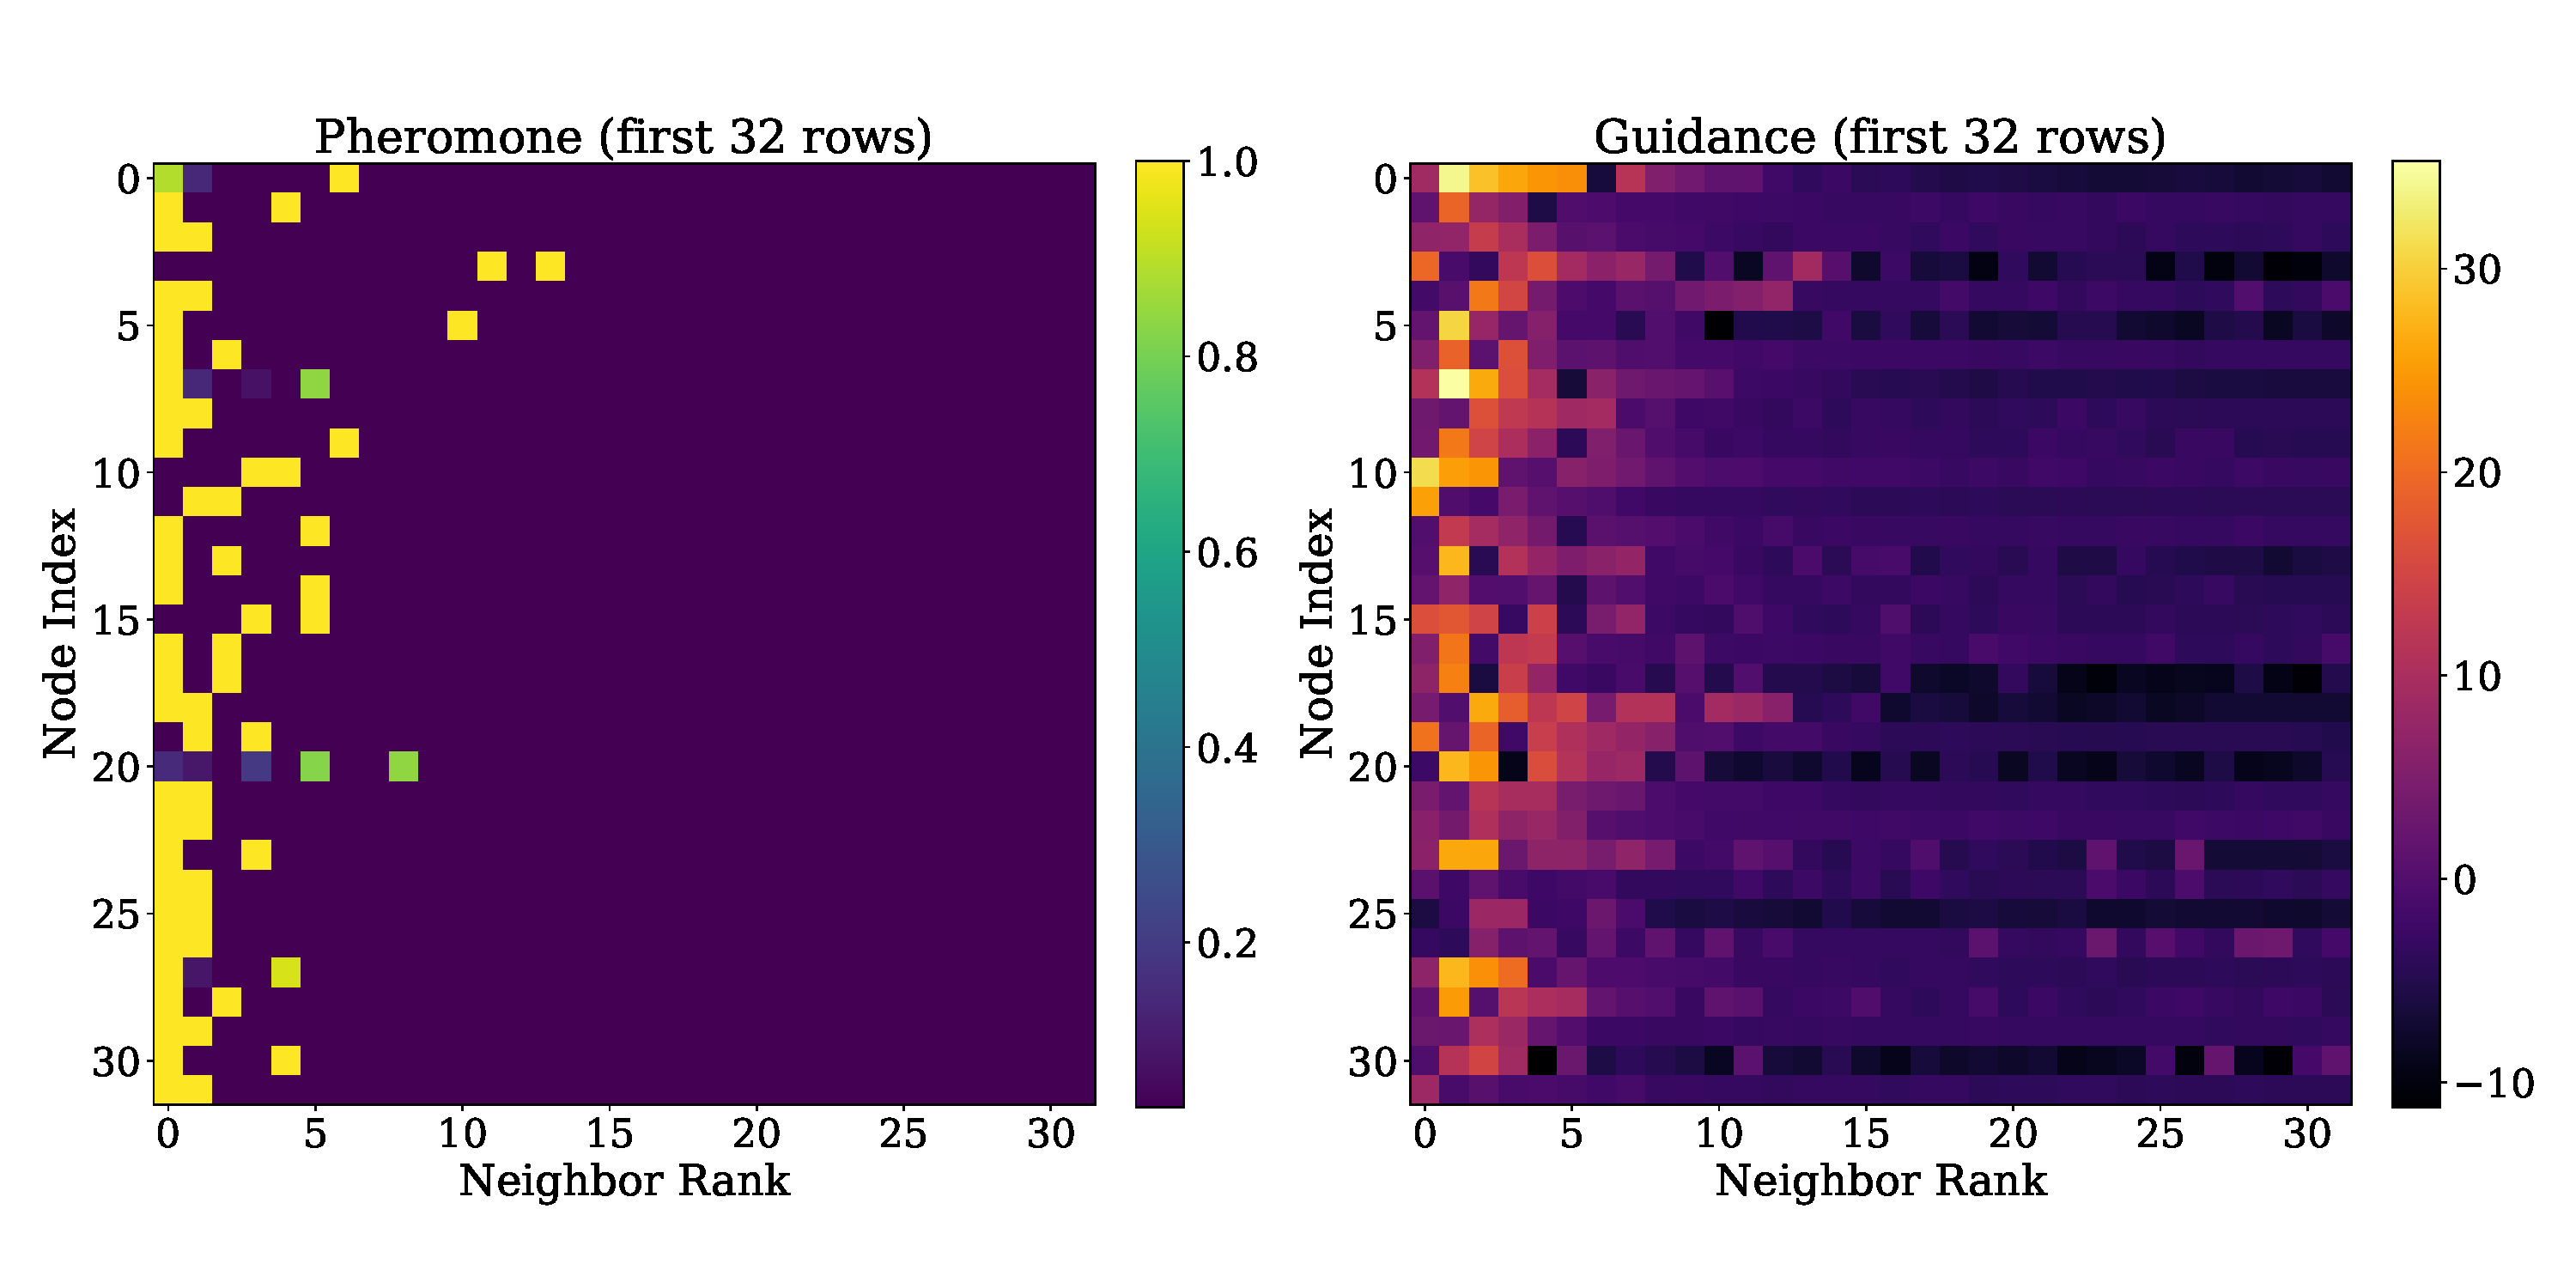
\includegraphics[width=\columnwidth]{figures/matrix_model_t5.pdf}
    \caption{Visualization of pheromone concentration and neural guidance scores (first 32 rows of the edge matrix) at successive iterations~$T$.}
    \label{fig:matrix_model}
\end{figure}

\smallskip\noindent\textbf{The policy learns to counteract ACO stagnation.}
Figure~\ref{fig:matrix_model} displays the pheromone matrix and corresponding neural guidance scores at successive iterations. As the search progresses, pheromone concentrations saturate and many edges converge toward $\tau_{\max}$, making the pheromone signal less informative. Despite this, the model outputs diverse guidance scores. In particular, over-reinforced edges often receive negative guidance, which redirects exploration away from stagnant regions. This selective counter-pressure is unavailable to static priors because they cannot observe the evolving pheromone landscape.

\smallskip\noindent\textbf{The 1K-trained model transfers zero-shot to larger synthetic scales.}
Table~\ref{tab:cross-scale} compares an in-scale model with the 1K-trained model on larger synthetic instances. The 1K model remains close to the in-scale model in all columns and is slightly better in two \TSP{}5K settings, providing scale-transfer evidence from a single trained policy.

\begin{table}[h]
\centering
\caption{Cross-scale zero-shot transfer: 1K model evaluated on larger instances.}
\label{tab:cross-scale}
\small
\renewcommand{\arraystretch}{0.80}
\begin{tabular*}{\columnwidth}{@{\extracolsep{\fill}}llcccc@{}}
\toprule
& & \multicolumn{2}{c}{$I_{1000}$} & \multicolumn{2}{c}{$I_{10000}$} \\
\cmidrule(lr){3-4} \cmidrule(lr){5-6}
Problem & Model & Gap & $\Delta$ & Gap & $\Delta$ \\
\midrule
\multirow{2}{*}{\TSP{}5K}
  & In-scale  & 1.30\% & --       & 0.75\% & --       \\
  & 1K model  & \textbf{1.23\%} & $-$0.07  & \textbf{0.72\%} & $-$0.03  \\
\midrule
\multirow{2}{*}{\TSP{}10K}
  & In-scale  & \textbf{1.59\%} & --       & \textbf{0.82\%} & --       \\
  & 1K model  & 1.66\% & +0.07    & 0.90\% & +0.08    \\
\midrule
\multirow{2}{*}{\CVRP{}5K}
  & In-scale  & \textbf{6.89\%} & --       & \textbf{3.36\%} & --       \\
  & 1K model  & 7.10\% & +0.21    & 3.60\% & +0.24    \\
\midrule
\multirow{2}{*}{\CVRP{}10K}
  & In-scale  & \textbf{11.04\%} & --      & \textbf{6.04\%} & --       \\
  & 1K model  & 11.72\% & +0.68   & 6.07\% & +0.03    \\
\bottomrule
\end{tabular*}
\end{table}

% \smallskip\noindent\textbf{\DyNACS{} generalizes zero-shot to real-world benchmarks.}
% Table~\ref{tab:realworld} evaluates the 1K-trained model on large TSPLIB and CVRPLIB instances without any fine-tuning. These instances include non-uniform, clustered, and geographically derived node distributions that differ substantially from the uniform training data. \DyNACS{} solves all instances and consistently improves over the unguided backend, confirming that the full guidance mechanism trained only on synthetic 1K instances can transfer to realistic benchmark distributions.

% \begin{table}[h]
% \centering
% \caption{Real-world benchmark results (zero-shot from 1K model, $I_{10000}$).}
% \label{tab:realworld}
% \small
% \renewcommand{\arraystretch}{0.80}
% \begin{tabular*}{\columnwidth}{@{\extracolsep{\fill}}lcccc@{}}
% \toprule
% & \multicolumn{2}{c}{TSPLIB (33)} & \multicolumn{2}{c}{CVRPlib (14)} \\
% \cmidrule(lr){2-3} \cmidrule(lr){4-5}
% Method & Gap (\%) & Time & Gap (\%) & Time \\
% \midrule
% LKH3 & 0.07 & 35m & 13.6 & 2.1h \\
% HGS & -- & -- & 5.15 & 5h \\
% \midrule
% LEHD~\cite{lehd}  & 13.2 & 38m & 16.9 & 40m \\
% GLOP~\cite{glop} & 6.99 & 34s & 20.6 & 39s \\
% SIL~\cite{sil} & 3.03 & 45m & 7.69 & 54m \\
% \midrule
% % ACO                   & 1.29 & 13s & 4.26 & 50.85s \\
% \textbf{\DyNACS{} (ours)}       & \textbf{0.89} & 11.57s & \textbf{3.66} & 51.07s \\
% \bottomrule
% \end{tabular*}
% \end{table}

\smallskip\noindent\textbf{Guidance--pheromone dynamics are consistent across scales.}
Figure~\ref{fig:guidance_pheromone_dynamics} shows a consistent two-phase interaction between neural guidance and pheromone. Early in the search, the policy tends to cooperate with pheromone by amplifying promising signals. Later, as pheromone concentrates and risks premature convergence, the policy increasingly suppresses over-reinforced edges to preserve exploration. The volatility diagnostics further show that guidance changes sharply after the first pheromone feedback, then settles into smaller but persistent updates across later outer steps. This rapid adaptation followed by steady refinement is expected from a policy that observes the search state directly: it reacts strongly when the pheromone field first becomes informative, then continues to recalibrate as the field evolves.

\begin{figure}[h]
    \centering

    \subfloat[Training correlation\label{fig:guidance_eta_corr}]{%
        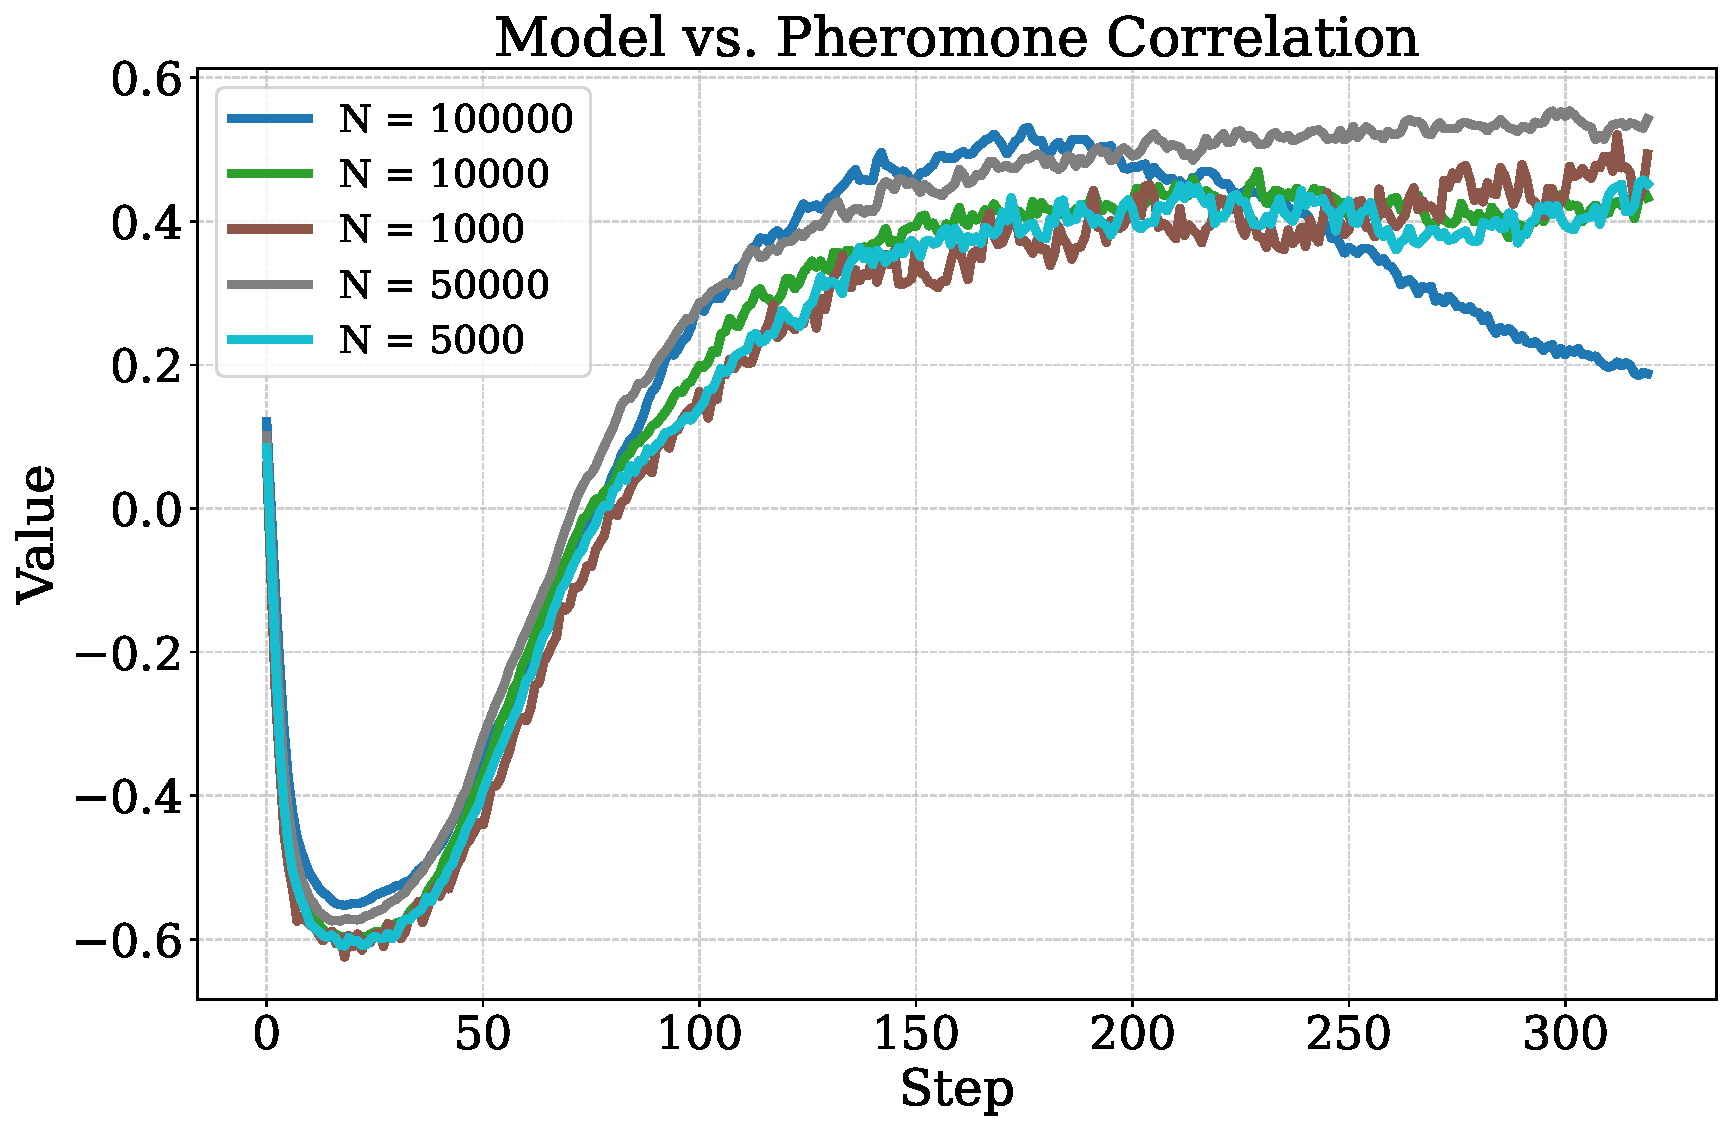
\includegraphics[width=.49\columnwidth]{figures/prior_eta_corr.pdf}%
    }
    \subfloat[Testing interaction\label{fig:interaction}]{%
        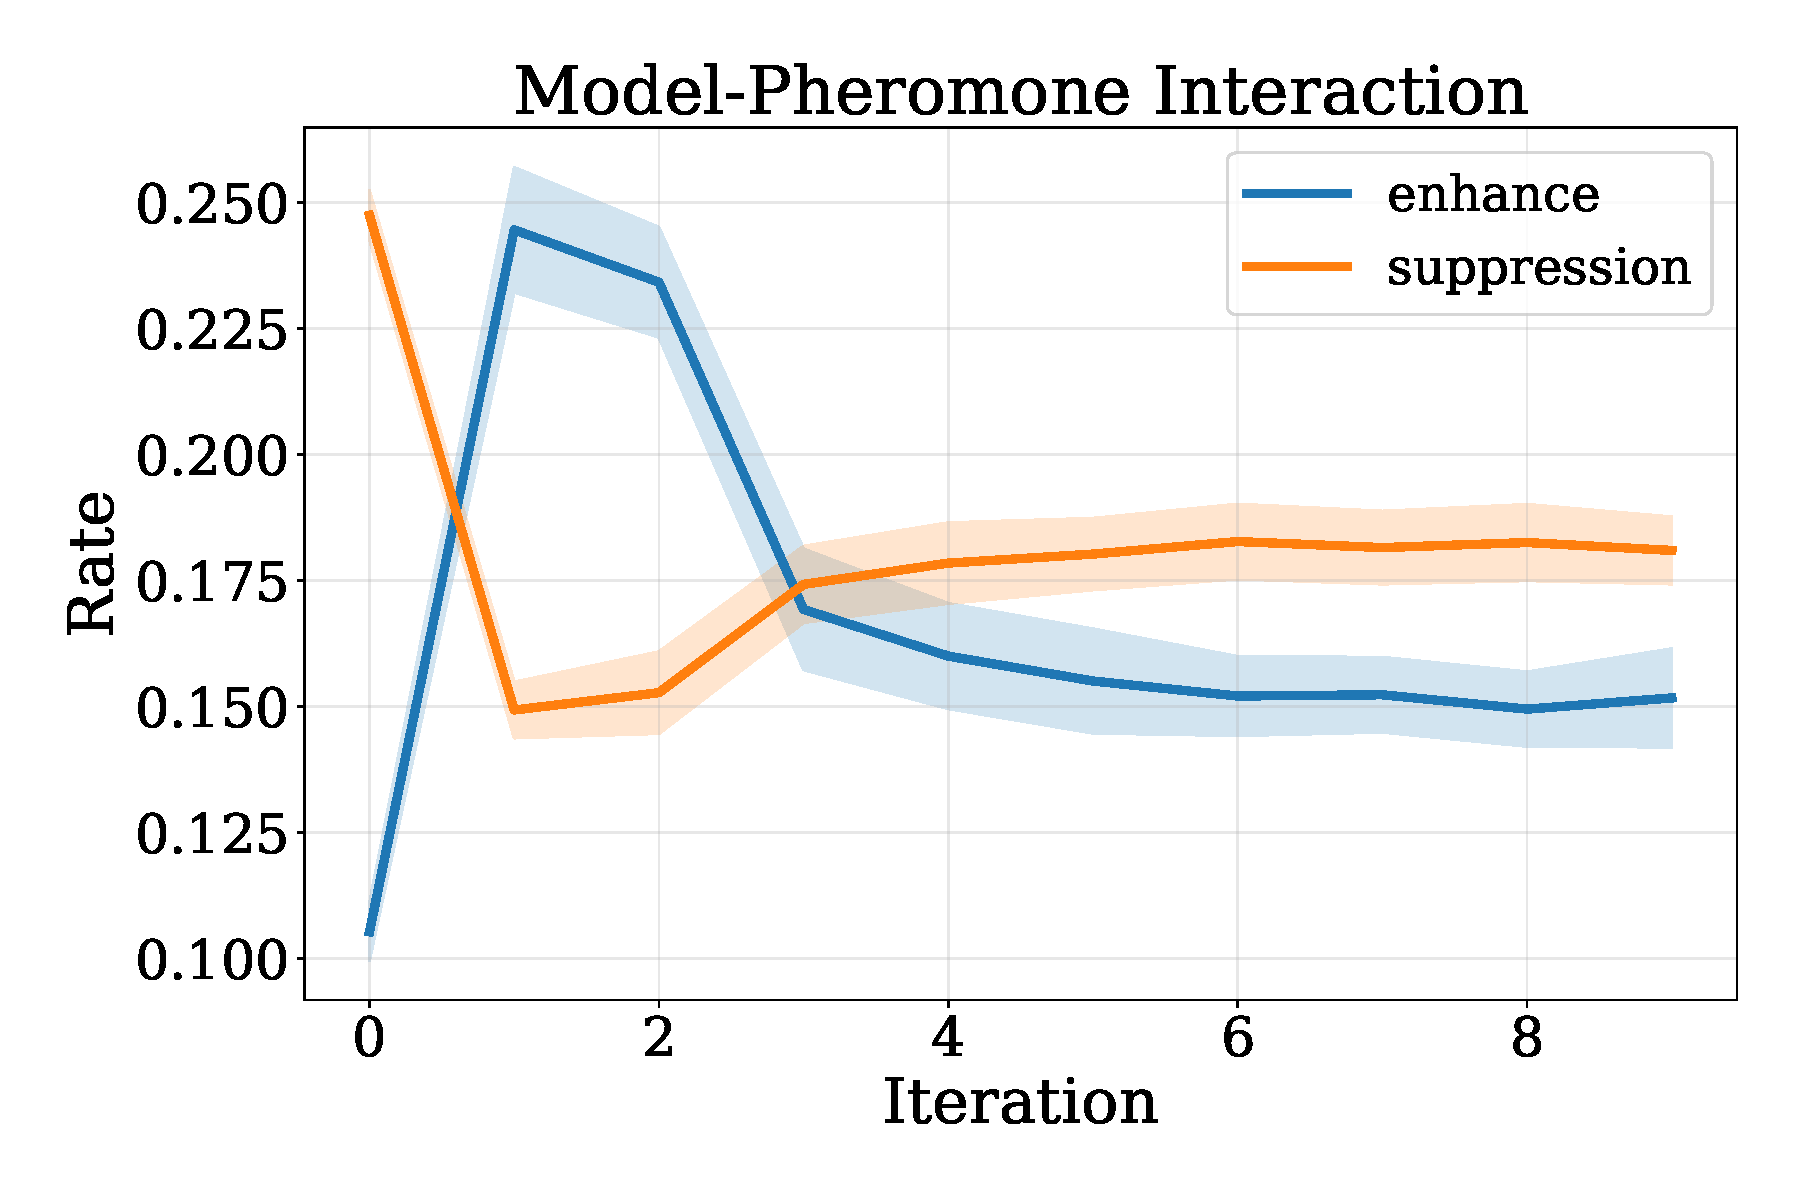
\includegraphics[width=.49\columnwidth]{figures/interaction.pdf}%
    }\hfill
    \subfloat[Guidance volatility\label{fig:prior_changes}]{%
        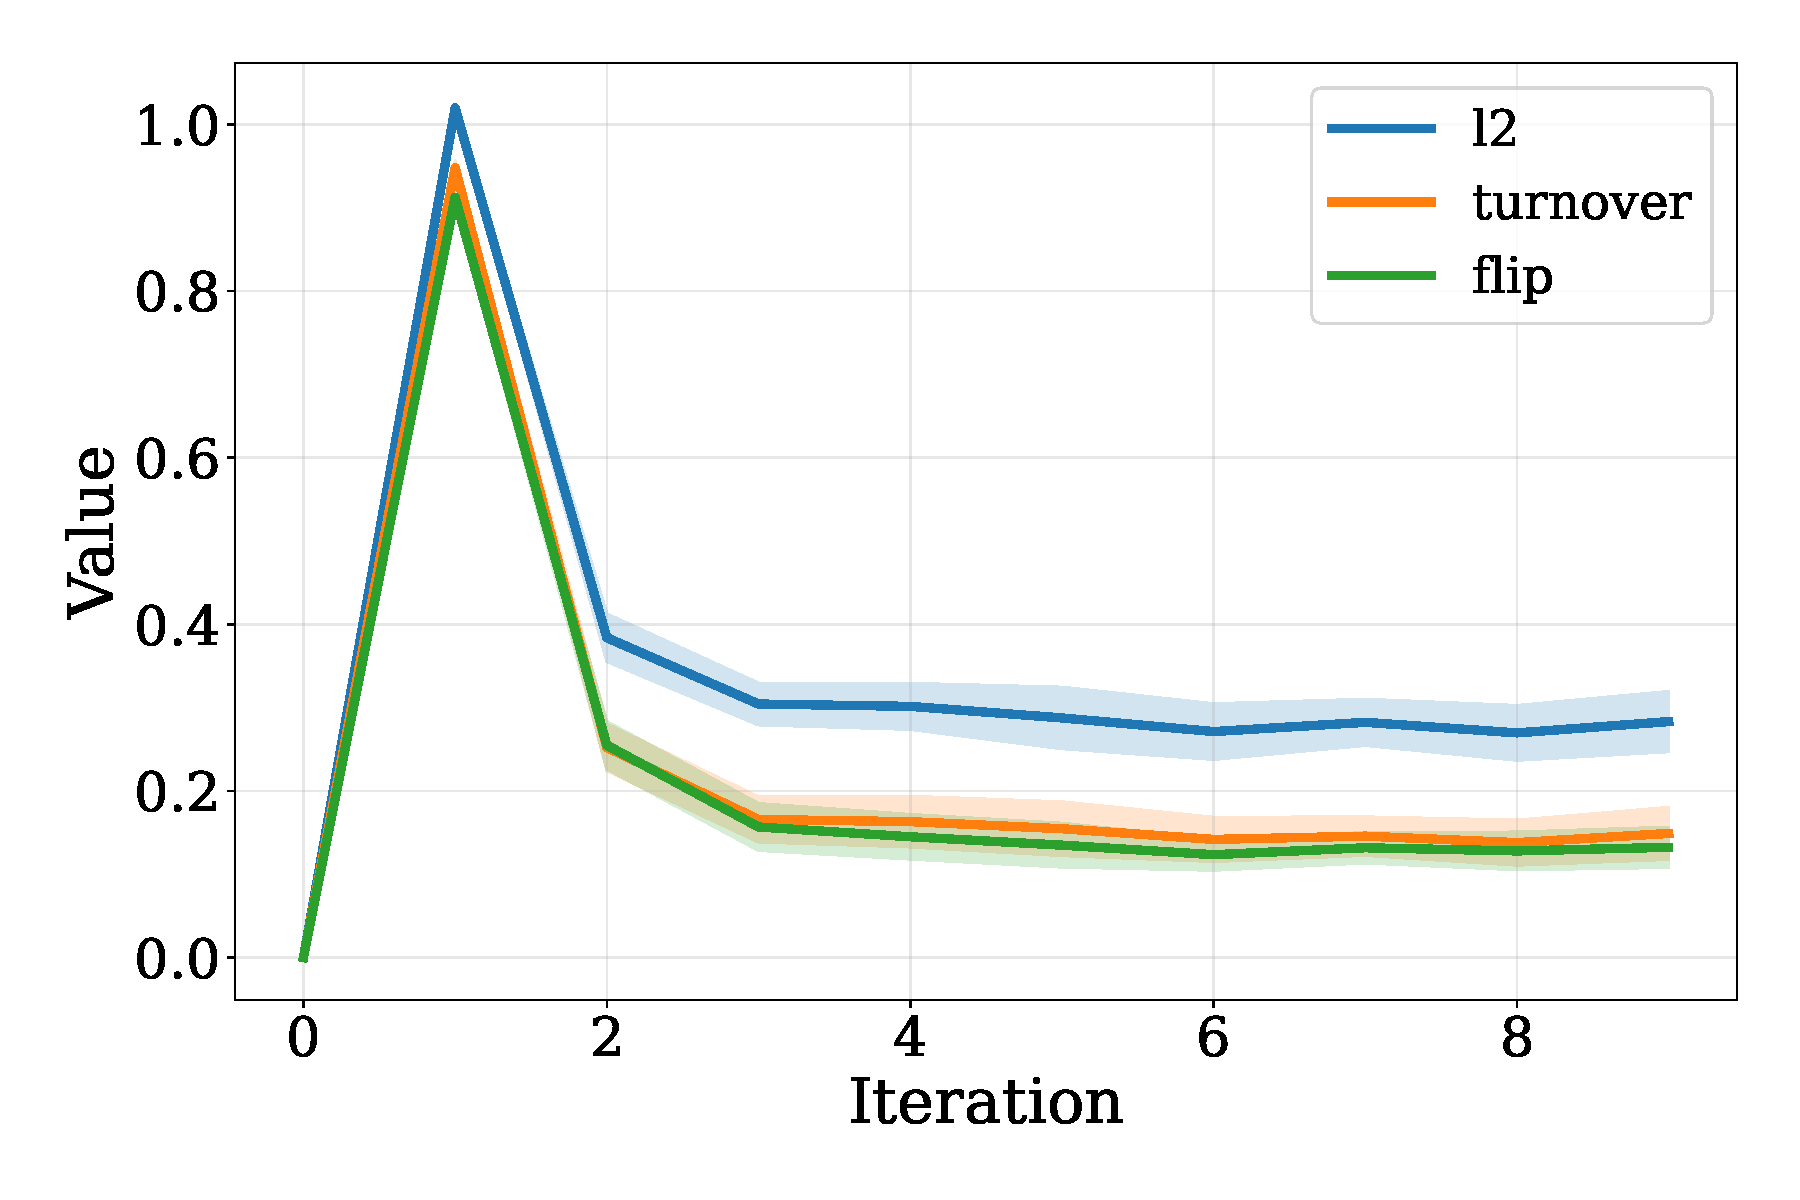
\includegraphics[width=.49\columnwidth]{figures/prior_changes.pdf}%
    }\hfill

    \caption{Visualization of the guidance-pheromone dynamics during both training and inference.}
    \label{fig:guidance_pheromone_dynamics}
\end{figure}
